\documentclass[12pt,a4paper,oneside]{report}
\usepackage[utf8]{inputenc}
\usepackage[T1]{fontenc}
\usepackage{amsmath}
\usepackage{amsfonts}
\usepackage{amssymb}
\usepackage{graphicx}
\usepackage{fontspec}
\usepackage{titlesec}
\usepackage{tocloft}
\usepackage[margin=2.5cm]{geometry}
\usepackage{lipsum}
\usepackage[skip=10pt]{parskip}
\usepackage{mwe,tikz}
\usepackage{tabto}
\usepackage{dashrule}
\usepackage[backend=biber,style=authoryear]{biblatex}
\usepackage{listings}
\usepackage{scrextend}
\usepackage{enumitem}
\usepackage{hyperref}

\ifdefined\EasyMarkPrivateBuild
	\input{private.tex}
	\newcommand{\IfPrivateBuild}[2]{#1}
\else
	\newcommand{\IfPrivateBuild}[2]{#2}
\fi

\addbibresource{citations.bib}

\setcounter{secnumdepth}{3}
\addtolength{\textwidth}{-1cm}
\addtolength{\oddsidemargin}{1cm}
\addtolength{\evensidemargin}{1cm}

\lstset{language=sh,basicstyle=\ttfamily}

% Calibri or sans-serif as default font
\defaultfontfeatures{Mapping=tex-text,Scale=MatchLowercase}
\IfFontExistsTF{Calibre}{
	\setmainfont{Calibre}
}{
	\renewcommand{\familydefault}{\sfdefault}
}

% TOC horizontal spacing
\cftsetindents{chapter}{0cm}{1cm}
\cftsetindents{section}{1cm}{1cm}
\cftsetindents{subsection}{2cm}{1.2cm}

% TOC vertical spacing
\renewcommand{\cftchapfont}{
	\bfseries
	\fontsize{13pt}{13pt}
	\selectfont
	\vspace{6pt}
}
\cftbeforechapskip12pt
\renewcommand{\cftsecfont}{
	\fontsize{11pt}{11pt}
	\selectfont
	\vspace{6pt}
}
\cftbeforesecskip6pt
\renewcommand{\cftsubsecfont}{
	\fontsize{10pt}{10pt}
	\selectfont
	\vspace{3pt}
}
\cftbeforesubsecskip6pt

% TOC title
\renewcommand\cfttoctitlefont{
	\hfill
	\fontsize{16pt}{16pt}
	\selectfont
	\bfseries
}
\cftbeforetoctitleskip6pt
\cftaftertoctitleskip12pt

% Title format for chapter, section, sub- and subsubsection
% See https://tex.stackexchange.com/questions/511981/titlesec-vertical-align-chapter-and-section
% The -5pt is just pixel pushing bc I couldn't figure out why my chapter/section/subsection/subsubsection headings are slightly indented
\titleformat{\chapter}[hang]{
	\normalfont
	\bfseries
	\filright
	\fontsize{16pt}{16pt}
	\selectfont
}{
	\makebox[1.7cm][l]{\thechapter}
}{0em}{}
\titlespacing{\chapter}{-5pt}{18pt}{12pt}

\titleformat{\section}[hang]{
	\normalfont
	\bfseries
	\filright
	\fontsize{14pt}{14pt}
	\selectfont
}{
	\makebox[1.7cm][l]{\thesection}
}{0em}{}
\titlespacing{\section}{-5pt}{18pt}{12pt}

\titleformat{\subsection}[hang]{
	\normalfont
	\bfseries
	\filright
	\fontsize{12pt}{12pt}
	\selectfont
}{
	\makebox[1.7cm][l]{\thesubsection}
}{0em}{}
\titlespacing{\subsection}{-5pt}{18pt}{12pt}

\titleformat{\subsubsection}[hang]{
	\normalfont
	\bfseries
	\filright
	\fontsize{11pt}{11pt}
	\selectfont
}{
	\makebox[1.7cm][l]{\thesubsubsection}
}{0em}{}
\titlespacing{\subsubsection}{-5pt}{12pt}{12pt}

\newcommand{\IncludeSchoolTemplate}[2]{
	\vspace*{-7em}
	\makebox[\textwidth]{
		\begin{tikzpicture}[
			every node/.style={anchor=north west,inner sep=0pt},
			x=1mm, y=1mm]
			\node (templatepage) at (0,0)
				{\includegraphics[width=\paperwidth,page=#1]{summary.pdf}};
			#2
		\end{tikzpicture}
	}
	\newpage
}

\newcommand{\SignatureLine}[1]{
	\vskip15pt
	\tabto{9cm}#1
	\vskip10pt
	\tabto{9cm}\hdashrule[0pt][x]{\fill}{.5pt}{.75mm}
}

\newcommand{\BlockCite}[2]{
	\begin{addmargin}[1cm]{0pt}
		#1

		\fullcite{#2}
	\end{addmargin}
}


\title{Easy Mark One}
\author{\IfPrivateBuild{\EmRealAuthorName}{T0astBread}}

\begin{document}
	\pagenumbering{gobble}
	\maketitle
	\IfPrivateBuild{
		\chapter*{Erklärung gemäß Prüfungsordnung}
		„Ich erkläre an Eides statt, dass ich die vorliegende Diplomarbeit selbstständig und ohne fremde Hilfe verfasst, andere als die angegebenen Quellen und Hilfsmittel nicht benutzt und alle den benutzten Quellen wörtlich oder sinngemäß entnommenen Stellen als solche kenntlich gemacht habe.“

		\EmPhysicalLocation, \today\tabto{9cm}{Verfasser*innen:}

		\SignatureLine{\EmRealAuthorName}
		\newpage
		\IncludeSchoolTemplate{1}{
			\node at (77,-28)
				{Informatik};
			\node at (77,-63)
				{\EmRealAuthorName};
			\node at (77,-80)
				{2019/20};
			\node at (77,-92)
				{Easy Mark One};
			\node at (77,-109)
				{\EmPartner};
			\node at (77,-127) [text width=305,align=justify] {
				\fontsize{12pt}{12pt}
				\selectfont
				\par
				Ziel des Projekts war die Entwicklung eines Tools zur Teilautomatisierung des Bewertungsprozesses für Programmier(haus)aufgaben in der Programmiersprache Java (Teilprojekt \emph{Automark}), sowie einer Web-Plattform für Lehrer und Schüler, um Informationen zu Aufgaben und Bewertungen zu teilen (Teilprojekt \emph{EasyMark}).
				\vskip10pt
				\par
				Alle Programme sollten in Java realisiert werden.
			};
			\node at (77,-174) [text width=300,align=justify] {
				\fontsize{12pt}{12pt}
				\selectfont
				\par
				Automark wurde als ein zusammenhängendes Java-Programm umgesetzt, das über die Kommandozeile sowie über eine GUI gesteuert werden kann. Diverse Libraries wurden für die zahlreichen Funktionen verwendet.
				\vskip10pt
				\par
				EasyMark wurde auf Basis des \emph{Javalin} Web-Frameworks entwickelt. Als Datenbank fungiert eine flache JSON-Datei mit Read/Write Lock. Für kryptographische Funktionen wurde Spring Security (als Standalone-Variante) verwendet.
			};
			\node at (77, -222) [text width=300,align=justify] {
				\fontsize{12pt}{12pt}
				\selectfont
				\par
				Automark: Die Teilaufgaben im Bewertungsprozess wurden zuerst implementiert, danach Nebenfunktionen wie Rollback/mark-resolved. Die GUI wurde entwickelt, um den Einstieg ins Programm zu erleichtern. Ebenfalls noch Zusatzfunktionen wie das automatische Versenden von Ergebnis-Emails und der Konfigurations-Wizard.
				\vskip10pt
				\par
				EasyMark: Zuerst wurden das Datenmodell und das Datenbanksystem entwickelt. Die Funktionalität würde zuerst abstrakt implementiert, dann die Business-Logic. Zuletzt wurde die Sicherheit des Servers überarbeitet und ein Programm zur Konfiguration eines Hosts geschrieben.
			};
		}
		\IncludeSchoolTemplate{2}{
			\node at (77,-28)
				{Informatik};
			\node at (77,-69){
				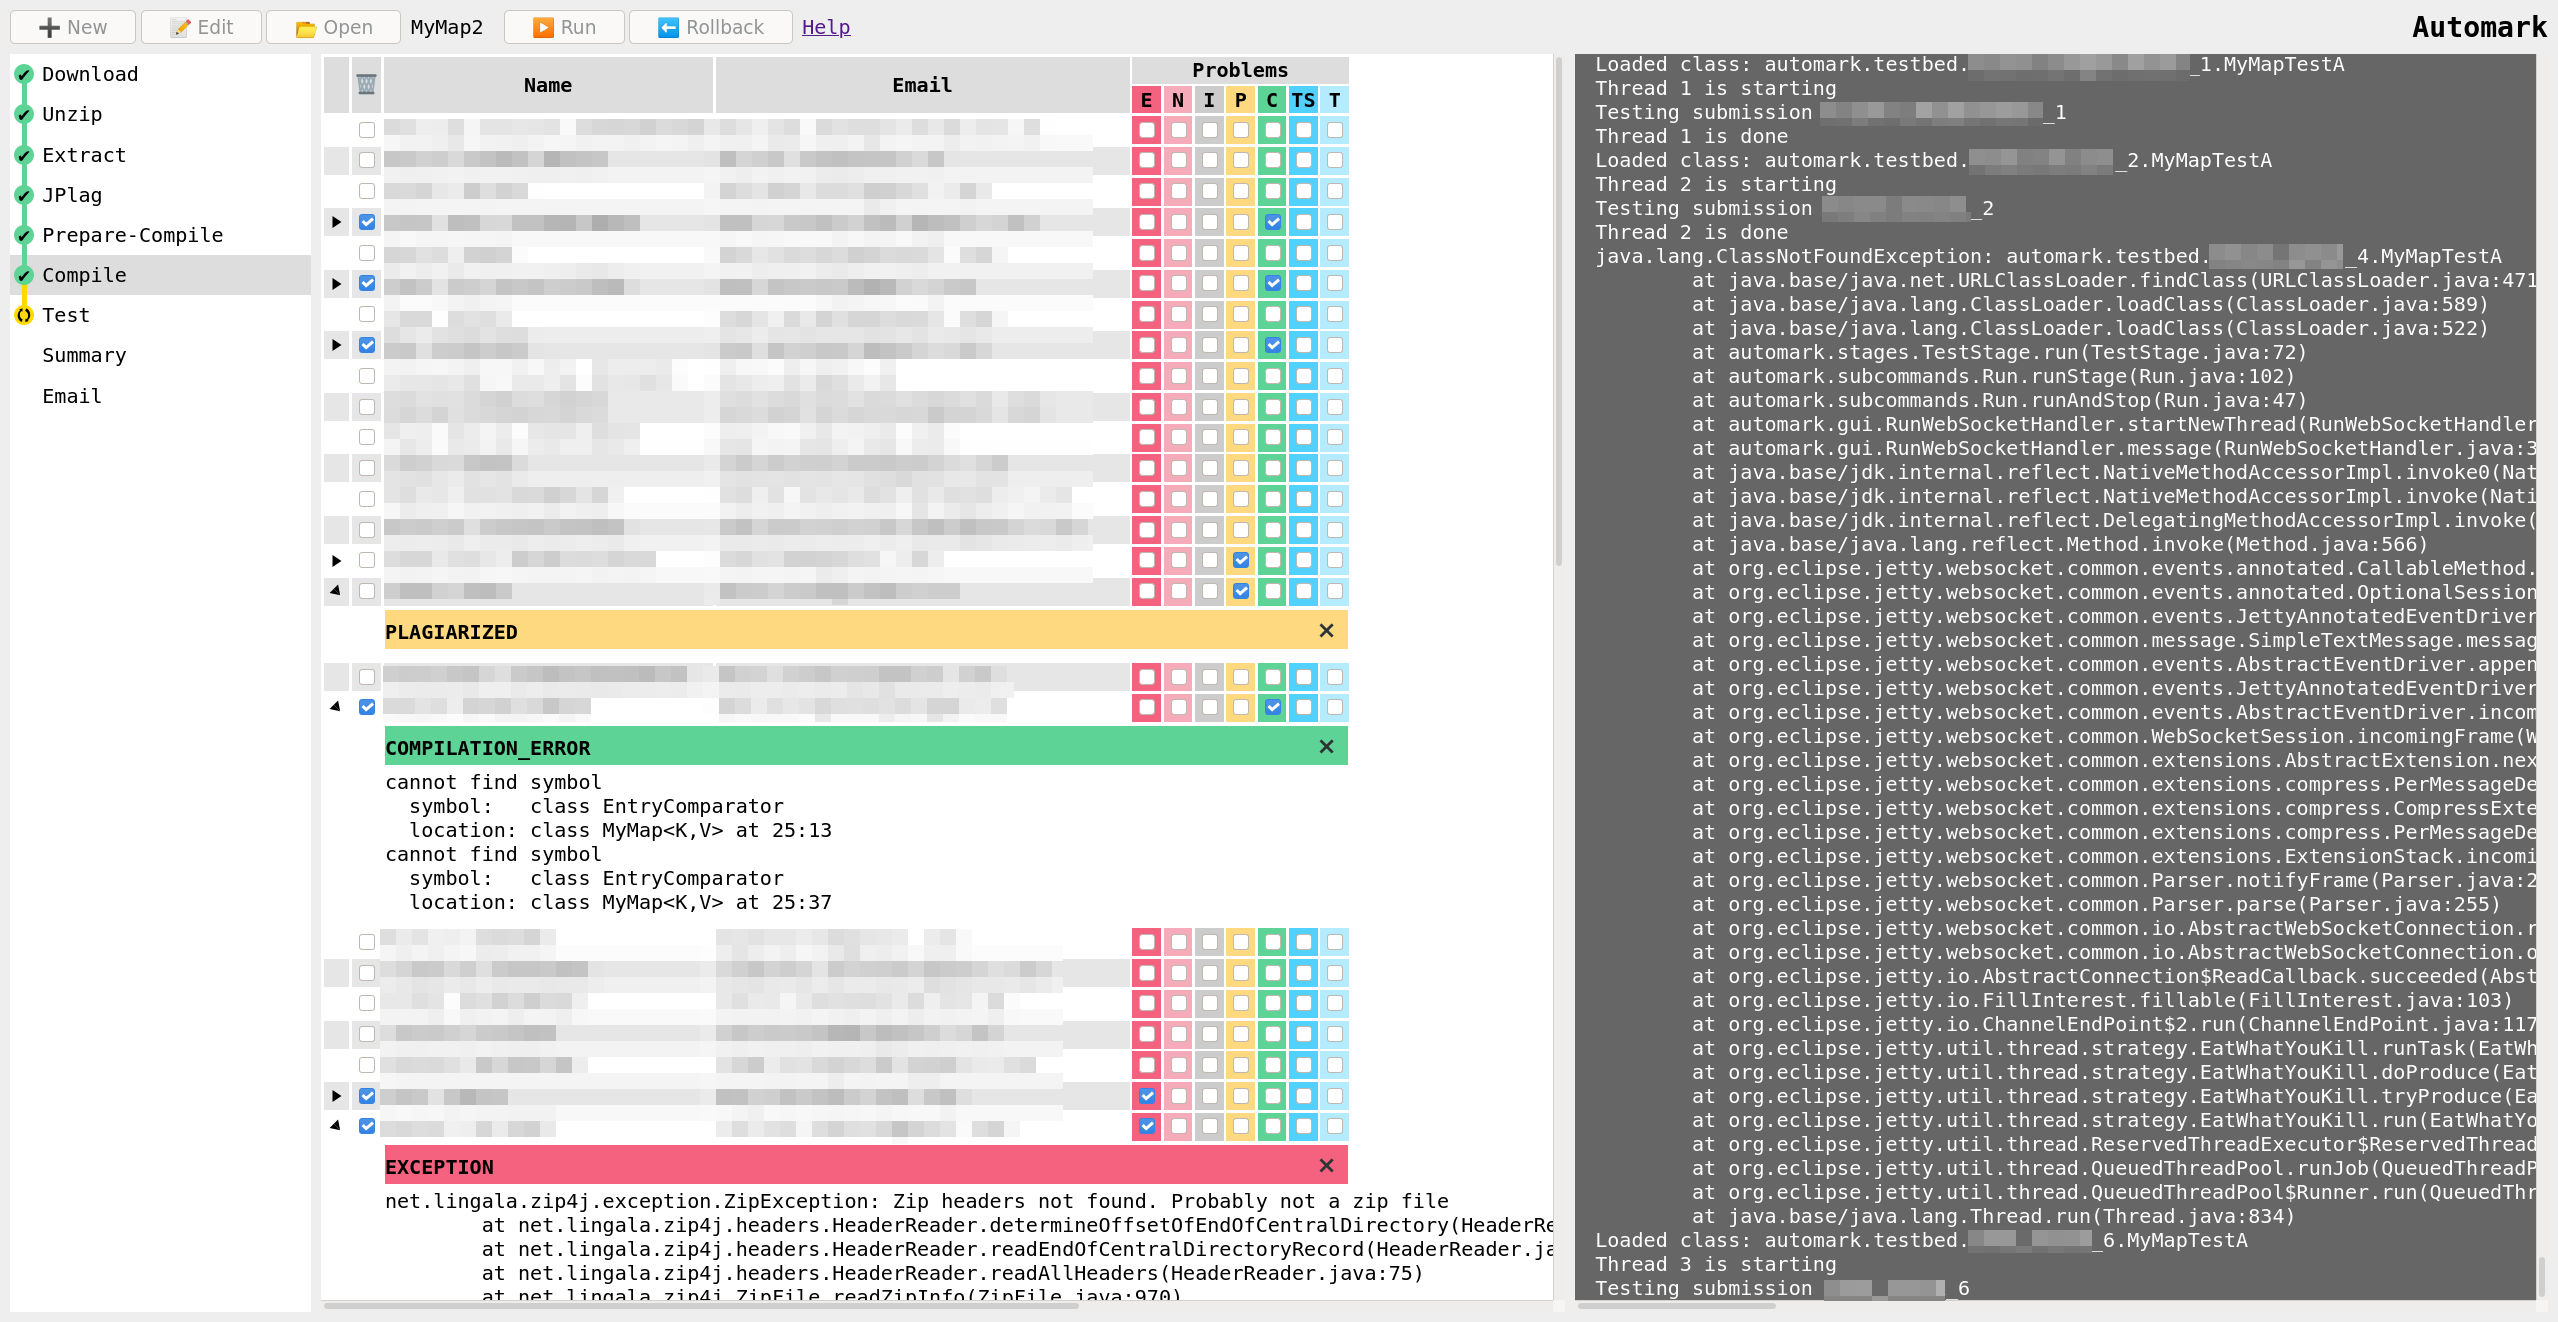
\includegraphics[width=310pt,trim=0pt 0pt 1110pt 0pt,clip]{automark_dashboard_w_details_expanded.png}
			};
			\node at (77,-171) [text width=305,align=center]
				{\emph{Screenshot der Automark-GUI (Ausschnitt). Links befindet sich eine Übersicht über alle Teilaufgaben im Prozess (\emph{Stages}), in der Mitte eine Tablle mit einer Übersicht sowie Details zu Schülerabgaben und deren Mängel. Persönlich identifizierbare Informationen sind unkenntlich gemacht.}};
			\node at (77,-220)
				{--};
			\node at (77,-239)
				{Öffentlich; Bibliothek der \EmSchoolName};
		}
		\IncludeSchoolTemplate{3}{
			\node at (76,-28)
				{Informatics};
			\node at (77,-63)
				{\EmRealAuthorName};
			\node at (77,-80)
				{2019/20};
			\node at (77,-92)
				{Easy Mark One};
			\node at (77,-109)
				{\EmPartner};
			\node at (77,-125) [text width=305,align=justify] {
				\fontsize{12pt}{12pt}
				\selectfont
				\par
				The project aimed to create a tool for partial automation of the grading process of programming assignments or homework in the programming language Java (subproject \emph{Automark}), as well as a web platform for teachers and students to share information on assignments and grades (subproject \emph{EasyMark}).
				\vskip10pt
				\par
				It was a requirement that programs be written in Java.
			};
			\node at (77,-173) [text width=300,align=justify] {
				\fontsize{12pt}{12pt}
				\selectfont
				\par
				Automark was realized as one self-contained Java program which can be controlled via the command line as well as over a GUI. Several libraries have been used to provide a number of different functionalities.
				\vskip10pt
				\par
				EasyMark was developed on top of the \emph{Javalin} web framework. A flat JSON file behind a read/write lock serves as a database. Spring Security (the standalone variant) provides cryptographic functionality.
			};
			\node at (77, -225) [text width=300,align=justify] {
				\fontsize{12pt}{12pt}
				\selectfont
				\par
				Automark: After basic tasks of the grading process, auxiliary functions like rollback/mark-resolved were implemented. A GUI was developed to ease the onboarding experience. The requirements were extended by additional functionality like the automatic sending of result email and the configuration wizard.
				\vskip10pt
				\par
				EasyMark: Initially, the database and the database system was implemented. Functionality was first implemented in the abstract, then the actual business-logic. Lastly the security of the server was revamped and a program to automatically configure a host was written.
			};
		}
		\IncludeSchoolTemplate{4}{
			\node at (76,-28)
				{Informatics};
			\node at (77,-64){
				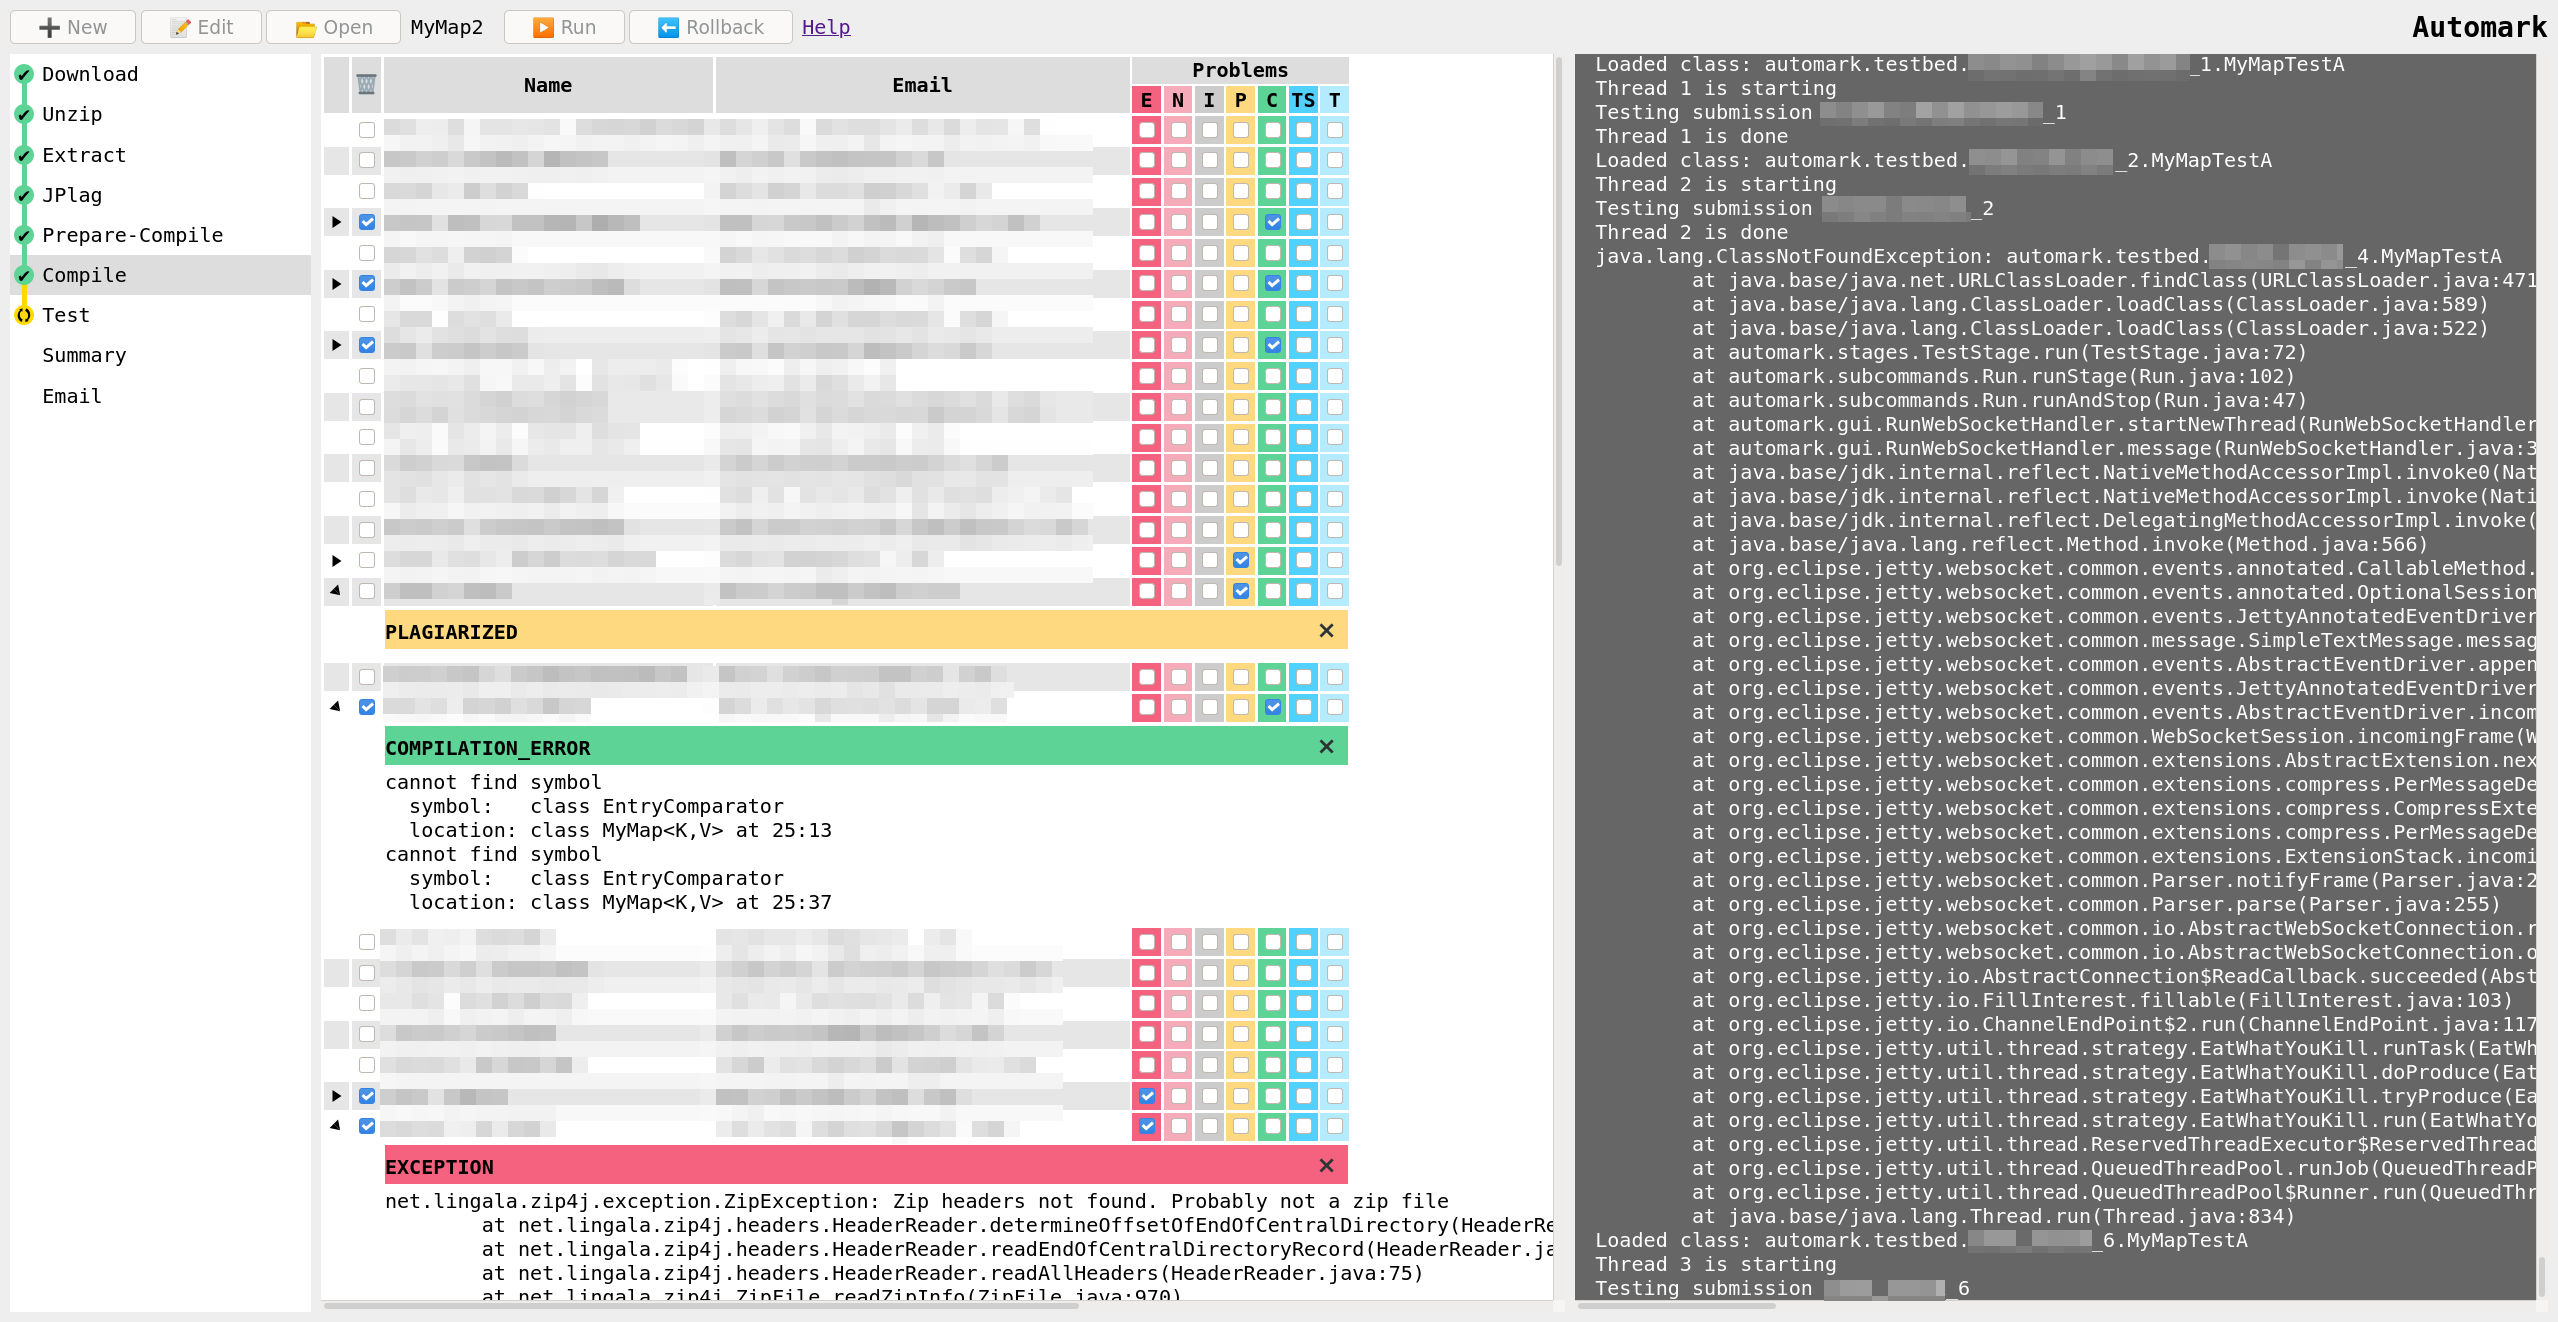
\includegraphics[width=310pt,trim=0pt 0pt 1110pt 0pt,clip]{automark_dashboard_w_details_expanded.png}
			};
			\node at (77,-166) [text width=305,align=center]
				{\emph{Screenshot of Automark's GUI (cropped). The panel on the left-hand side displays an overview over all tasks in the process (\emph{stages}). In the middle there's a table showing an overview as well as detailed information about students' submissions and any problems with them. Personally identifiable information has been blurred.}};
			\node at (77,-220)
				{--};
			\node at (77,-240)
				{Public; Library of the \EmSchoolName};
		}
	}{}
	\clearpage
	\tableofcontents
	\newpage
	\pagenumbering{arabic}
	\chapter{Introduction}
	The Easy Mark One project originated from a dissatisfaction with the workflow of reviewing, grading and communicating assignments in programming classes. Workflows to this date are largely based on repetitive manual labor and rigor which not only makes them error-prone; it also results in many teachers outright (and understandably) skipping this work which can create a net negative for the pupils' education.

	The project aims to fix this issue with two independent software packages: \emph{Automark} and \emph{EasyMark}. Both programs are implemented largely in Java and some other languages like JavaScript, CSS and Pebble\parencite{pebblewebsite} for web-based components.

	\section{Automark}
	Automark is a tool to automate the objective tasks of grading programming assignments. That means it can automatically download, verify, compile and test programming assignment submissions and generate summaries and reports about the status of each submission along the way.

	To achieve its goals of simplicity and high automation, Automark integrates with existing learning management systems (LMS), third party verification tools, compilers and other systems. Despite its deep integration, Automark is built to be highly resilient against failure. The program can handle invalid submissions and unexpected input without crashing; instead it associates errors with the submission it has been processing and notifies the operator and -- optionally -- also the submitter about it.

	Automark employs advanced and up-to-date third party tools for testing and detecting software plagiarism between submissions. In addition to that, it automatically builds a historical database of all submissions for a given assignment to detect plagiarism from previous years' submissions.

	Automark replaces a range of existing tools for its tasks and employs a clean and extensible internal structure. It is perfect for tying together unorganized manual grading workflows.

	\section{EasyMark}
	EasyMark is an online web-based platform for connecting students and teachers and communicating grades and assignment information.

	EasyMark provides teachers with the ability to create courses with chapters and assignments for students to view. Then later on, when a student has completed an assignment and submitted it over another channel (such as Moodle) the teacher can perform an assessment of the submission (for example, via Automark) and enter the results in a user-friendly yet powerful GUI on EasyMark. EasyMark then automatically calculates the new grading status of then student and notifies them the next time they log in.

	Additionally, EasyMark allows students to volunteer for an exam on chapters where the teacher has enabled the feature. The teacher is able to view these test requests on a feature-rich dashboard immediately after logging in.

	Unlike Automark, EasyMark does not aim to replace existing tools (which in this case would be learning management systems like Moodle or WebUntis). Rather, it extends them with new features not available in currently employed LMS solutions and fosters cooperation with existing systems by providing functionality to link to and import from third party platforms such as Moodle.

	EasyMark also employs unparalleled security and data protection features. Personally identifiable information (such as names) are encrypted and only accessible via the teacher's access token. Bad actors who gain access to the server are not able to read the protected information from the database file. In addition to that, EasyMark gives teachers and students deep insight over what happens to their accounts. Teachers and students have the ability to view and revoke currently active sessions on their account. Teachers also see an append-only log of all actions conducted with their account to quickly detect intrusion.

	\iffalse
	\chapter{Quick-Start Guide}
	This chapter is for readers who would like to have a quick development setup for review and assessment. It does not go into detail about the various features of the programs described and the end-result is not ready to be used in a production environment. For production-ready builds and deployment please see one of the later chapters. %TODO: reference production-ready build/deploy chapters

	The guide will often mention an "IDE" (integrated development environment). It should be noted that you do not require an IDE to complete this setup, although it is advisable. The guide sometimes includes special setup instruction for IntelliJ IDEA\parencite{intellijwebsite} hence why it is the recommended IDE for this guide.

	\section{Automark}
	This section guides you through the setup of Automark for development and assessment.

	\subsection{Obtaining the Source}
	The Automark source code can be obtained from the project's GitHub repository using the builtin functionality to clone (download) repositories using the version control system (VCS) Git. Additionally you can use the command line ("Git Bash" on Microsoft Windows, any shell on other systems) with the following command:
	\begin{lstlisting}[language=sh]
		git clone https://github.com/T0astBread/automark
	\end{lstlisting}
	The author does not guarantee availability of the source code repository at this location.

	If you have access to the physical copy of this document you can also obtain the source from the included DVD-ROM.

	\subsection{Opening the Project}
	You can open the project as a normal Gradle project. In IntelliJ IDEA this is the "Open or Import" option on the start screen or the "Open..." option in the "File" dropdown on any other screen. After opening the project a notification will pop up with a link titled "Import Gradle project". Click that link.

	\subsection{Running the Program}
	When running Automark you have two choices: You can use it from the command line or you can use it via the included GUI. To set up a new project or explore features it is recommended you use the GUI, since it provides a simple UI for project creation, configuration and usage.

	\pagebreak
	To run the program you can execute the Gradle task "run" with special options depending on how you intend to run the program. On the command line this can be done with
	\begin{lstlisting}[language=sh]
		./gradlew run --args "<automark args go here>"
	\end{lstlisting}
	in the project directory. On Windows replace "gradlew" with "gradlew.bat".

	You can create an IntellJ IDEA run configuration to execute the task with a single keystroke. To do so, click "Add configuration..." or (if you already have run configurations) click the run configuration drop down and click "Edit configurations...". In the new window, click the plus icon in the top left corner and select "Gradle". In the "Gradle project" field enter "automark", leave the "Task" field blank and instead enter \lstinline|run --args "<automark args go here>"| in the "Arguments" field. Details of the various command line arguments can be found in later chapters. %TODO: reference Automark command line arg chapters

	It is recommended you enter \lstinline|-Dfile.encoding=UTF8 -Dsun.jnu.encoding=UTF-8| in the "VM Options" field to ensure HTML content is rendered correctly for web features.

	To quickly try out features, it is recommended you start the GUI. The subcommand for that is simply "gui" (\lstinline|run --args "gui"|). If your platform supports it (which should be the case for Windows) a browser window will pop up titled "Automark". If your platform lacks support for the Java feature used to implement that an URL will be printed to stdout which you can open in your browser.

	\textbf{Important:} For security reasons, Automark will set a cookie in your browser when you start it and deny requests from browsers that do not have this cookie. You can't use Automark from a browser window or tab other than the one it opened in. If you close that window or tab, you would have to restart the Automark GUI to use it again.

	%TODO: continue this if needed or delete
	\fi

	\chapter{Automark}

	\section{Technology Used}
	Automark is implemented on top of Java and incorporates various libraries to provide some of its functionality. It has been written using the IntelliJ IDEA IDE and the Gradle build system.

	\subsection{Java}
	Java is a class-based, object-oriented programming language that runs on its own virtual machine (VM) called the JVM and can thus run on any operating system that implements a JVM\parencite{oraclethejavalangenvironment}. The technology was chosen because of the familiarity of the author and the cooperation partner with the language and the (in the field of programming) well-known stability of the language.

	\subsection{Gradle}
	Gradle is a system to automate compilation, linking and packaging (in combination referred to as "building") for a variety of languages including Java. In addition to simplifying software builds it also caches results and avoids re-compiling up-to-date compilation units (classes in Java). Gradle is also well-integrated into the IDE used.\parencite{gradlewebsite}

	\subsection{IntelliJ IDEA}
	IntelliJ IDEA is an integrated development environment (IDE) from JetBrains s.r.o.\parencite{intellijwebsite} An integrated developmentcan be viewed as an advanced text editor that offers convenience features for the programmer, such as syntax highlighting, context-aware code completion, debugging and build integration\parencite{stevenjzeilintegrated}\parencite{idewikipedia}. IntelliJ was chosen because of the author's familiarity and satisfaction with it. The Apache-2.0-licensed Community edition was used.

	\subsection{Libraries}
	Automark uses a few libraries to provide some of its functionality.

	\subsubsection{GSON}
	GSON is a Java library by Google for simple serialization and deserialization of Java objects to and from JSON objects and arrays\parencite{gsongithub}. It was chosen since it operates using Java's reflection feature which spares the developer from having to write explicit parsing code.

	\subsubsection{JSoup} \label{sec:jsoup}
	\BlockCite{jsoup is a Java library for working with real-world HTML. It provides a very convenient API for fetching URLs and extracting and manipulating data, using the best of HTML5 DOM methods and CSS selectors.}{jsoupwebsite}

	JSoup is used for automatically obtaining data from Moodle. Since the Moodle version Automark is built for does not make heavy use of client-side scripting (which JSoup does not support), JSoup was the most stable choice.

	Alternatives to JSoup would typically use a fully-fledged browser such as Google Chrome or Firefox and automate website interactions using APIs (application programming interfaces) provided by the browser which then perfoms interactions as if a human user had done it. Aside from reduced speed, the main drawback with this approach is that library versions quickly become outdated due to the underlying browser version becoming outdated. In the case of some libraries, vendors will not provide downloads for old browser versions anymore leading to breakage of new installations.

	\subsubsection{Zip4j}
	Zip4j provides ZIP packing and extraction functionality.\parencite{zip4jwebsite} It is used to unpack submission files downloaded from Moodle or provided by the operator.

	\subsubsection{JUnit 5}
	JUnit 5 is a unit testing framework for JVM languages.\parencite{junit5website} In Automark it is used for running unit tests provided by the operator against students' submissions. JUnit 5 provides a simple interface for automating test execution via the "junit-platform-launcher" package\parencite{junitplatformlauncherdocs}.

	\subsubsection{Simple Java Mail}
	Simple Java Mail wraps Java's email APIs to improve the developer experience (DX) when sending email\parencite{simplejavamailwebsite}. It is used to send result-email to students after their submissions were tested if enabled by the operator.

	\subsubsection{Spark}
	Spark is a web server framework for JVM languages (with special focus on Java and Kotlin)\parencite{sparkwebsite}. It is used to provide the in-Browser GUI locally and with security restrictions. %TODO: refenrence GUI security restrictions chapter

	\section{Functionality}
	Automark is used to automate the process of grading programming assignments in the programming language Java as far as possible and with superior stability. To facilitate this, Automark employs a design that seperates the process of reviewing assignments (called "pipeline") into multiple tasks (called "stages"). Each stage is dependent on the result of the respective previous stage.

	Stages are run without manual intervention unless required. If a submission fails to fulfill the requirements of a stage, it will be tagged with a so-called "problem" and possibly excluded (if the specific problem renders the submission unfit for further processing). If a stage completes, Automark will automatically continue with the next stage, unless a problem has been detected in at least one submission during the stage.

	After a stage completes with new problems in submissions the operator should review the problems and do one of the following to each:
	\begin{itemize}
		\item \textbf{Leave the problem be} if it is justified.
		\item Use the \textbf{Rollback} feature to revert the completed stage. The operator can then adjust the output of the previous stage to correct any mistakes that cause the stage to output unwanted problems.
		\item Use the \textbf{mark-resolved} subcommand to remove one or more problems from the database without actually changing the submission data.
	\end{itemize}

	\subsection{Problems}
	Automark categorizes failures of submissions to meet requirements as problems of different types.

	\begin{description}[align=left]
		\item[EXCEPTION] Denotes that a Java exception was thrown while processing the submission. This most frequently occurs due to invalid or malformed input in submissions.
		\item[NOT\_SUBMITTED] Denotes that while it was captured that the student has been added to the assignment the student did not submit a solution.
		\item[INVALID\_SUBMISSION\_FILE] Used to report a variety of problems with the submission file(s) that were not captured as a Java exception during processing.
		\item[PLAGIARIZED] Denotes that a submission contains similarities with another submission of the same assignment or a submission of the assignment from a previous year. This problem type is not assigned automatically. See plagiarism detection. %TODO: reference plagiarism detection chapter
		\item[COMPILATION\_ERROR] Denotes that the Java compiler reported one or more errors while compiling the source files in the submission. If the compiler reports errors while compiling the operator-provided test suites with the sources it is not reported as a \lstinline|COMPILATION_ERROR| but rather as a \lstinline|TEST_SUITE_FAILURE|.
		\item[TEST\_SUITE\_FAILURE] Denotes that, during the \lstinline|TEST| stage, a whole test suite either was not completed (for example due to a timeout) or was not started in the first place (for example due to a compilation error).
		\item[TEST\_FAILURE] Denotes a failure of a JUnit test during the \lstinline|TEST| stage on the given submission.
	\end{description}

	In addition to the type a problem also includes a summary which contains either a short description or detailed diagnostic information such as a stacktrace. In case of the latter it will be shortened in reports sent out to students. Problems also record in which stage they occured.

	\subsection{Stages}
	Automark seperates the processing pipeline into nine stages. This section enumerates the stages and explains their implementation.

	\subsubsection{Download}
	The \lstinline|DOWNLOAD| stage is not an actual stage but rather a hyperonym to refer to either the \lstinline|BypassDownloadStage| or the \lstinline|MoodleScraperStage|. The whole program refers to them using the term \lstinline|DOWNLOAD| with the only exception being the configuration wizard.

	\subsubsection{MoodleScraperStage}
	This stage takes Moodle credentials (of the operator) as its parameters among others. It logs into Moodle, obtains the names and email addresses of students added to the assignment and checks if a submission is present. If it is, it is downloaded. If it is not, a \lstinline|NOT_SUBMITTED| problem is added to the submission entry for the student and it is excluded from further processing.

	The web scraping features in this stage are implemented using the JSoup library (see \ref{sec:jsoup}~JSoup). JSoup is augmented to store cookies from server responses to implement sessions.

	\subsubsection{BypassDownloadStage}
	This stage is an alternative to the \lstinline|MoodleScraperStage| and is mainly designed as an emergency solution if the \lstinline|MoodleScraperStage| breaks, for example due to an incompatible change in the Moodle website.

	The \lstinline|BypassDownloadStage| obtains submissions and metadata from a ZIP file which the operator can download from Moodle manually using the "Download all submissions" ("Alle Abgaben herunterladen" in German) option in the grading editor.

	The stage optionally reads in a file called "emails.csv" which is a comma-seperated values file in the format \lstinline|Moodle name;email address| which it uses to map email addresses to submissions for potential later use in the \lstinline|EMAIL| stage. The lines in the file do not have to map exactly to the names in the "all submissions" ZIP file.

	Normally the \lstinline|BypassDownloadStage| does not mark missing submissions as \\\lstinline|NOT_SUBMITTED| since the "all submissions" ZIP file from Moodle does not contain any information from which the stage could infer that a student who has not submitted a solution exists. However, if an "emails.csv" file is present and the file contains one or more lines with names that do now match any submission, then the \lstinline|BypassDownloadStage| will create submission entries for those students, mark them as \lstinline|NOT_SUBMITTED| and exclude them from further processing.
\end{document}
